% \cleardoublepage
\chapter{Plan and Timeline}\minitoc\label{sec:plan}\vspace{.5cm}

This chapter will outline our project plan and provide a timeline for its execution.

\section{Project Plan}

\begin{figure}[H]
	\centering
	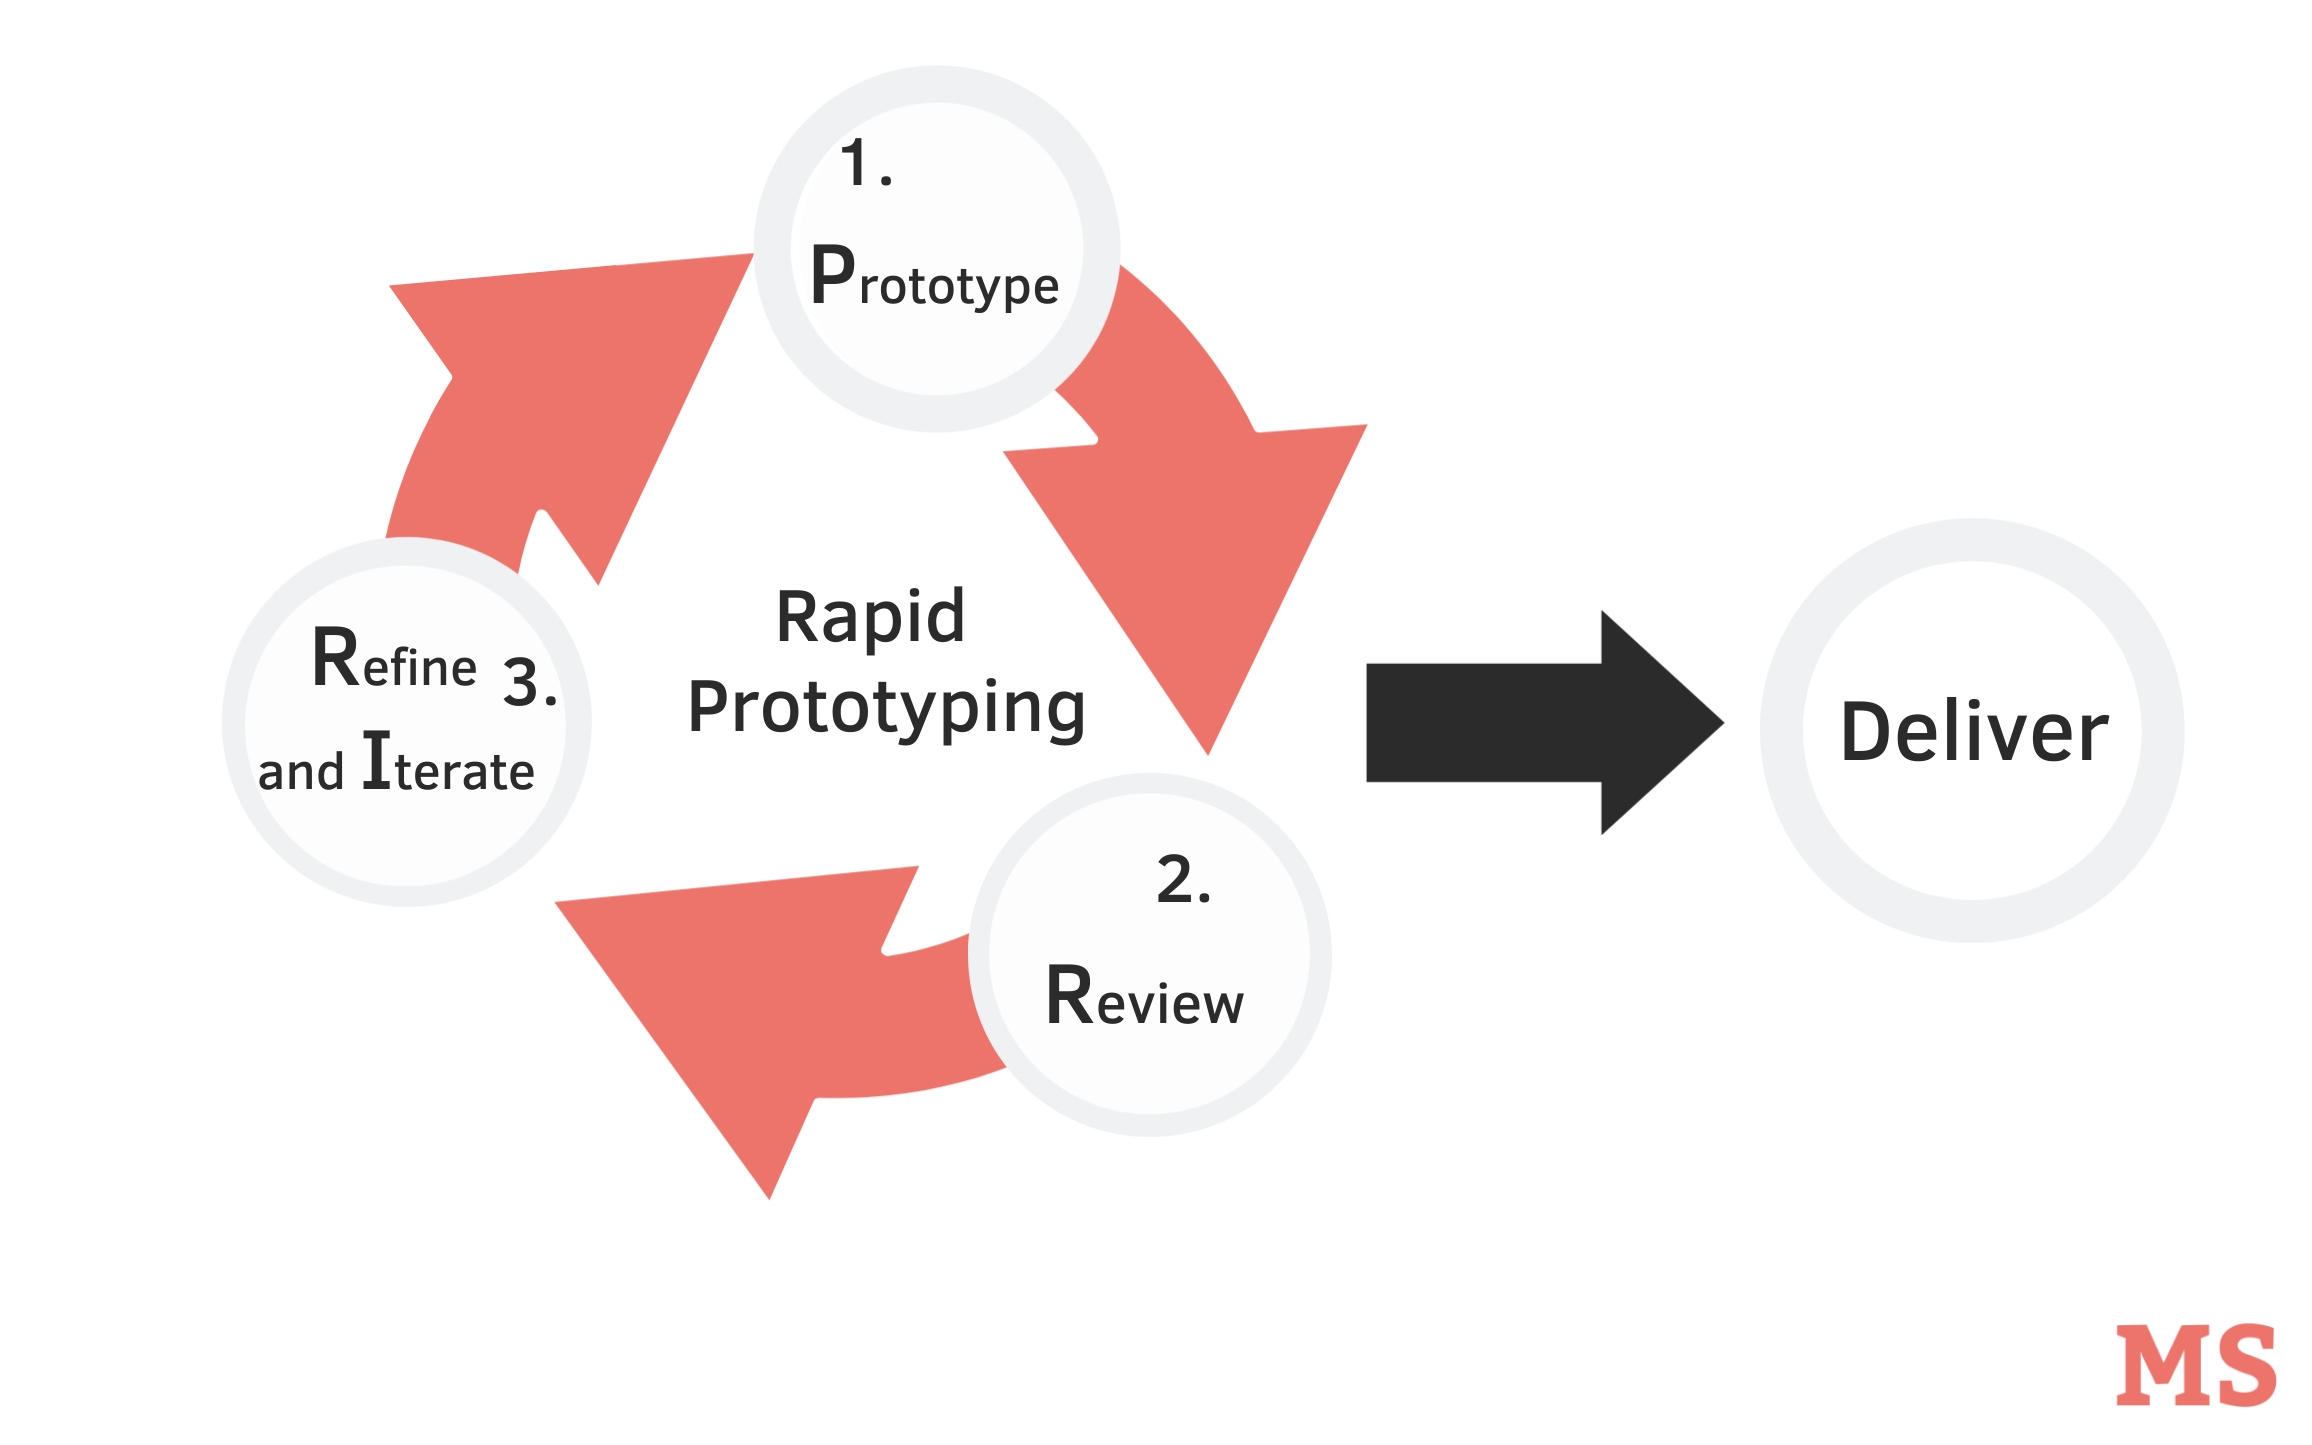
\includegraphics[width=0.6\textwidth]{rapid_prototyping_software.png}
	\caption{Rapid prototyping cycle \cite{marketsplash_rapid_2021}}
	\label{fig:plan:rapid_prototyping_software}
\end{figure}

During the development phase, we adhere to the rapid prototyping model (\Cref{fig:plan:rapid_prototyping_software}). 
The development process follows a loop of building prototypes, reviewing them, refining the implementation, and iterating on the design. 
Features and components are broken into  self-contained and independent tasks, each can be completed within a time frame of 1-2 weeks.
\\


The thesis is set to be completed in 6 months (\Cref{fig:plan:TIMELINE}), divided in 3 phases: \textbf{Prototype Building}, \textbf{Feature}, and \textbf{Refinary and Test}.
The library's development is expected to span a period of 3 months. 
During the initial month, the focus will be on creating the core features of MTX. 
These features involve tasks such as packet exchange with XDP socket, collecting and delivering packets from applications, and inspecting packets for flow control purposes. 
The subsequent 4 weeks will be dedicated to refactoring and shaping the library, ensuring it meets the necessary requirements for packaging and distribution. 
Following this, the third month will be allocated to constructing the control and data plane to support various configurations. 
After completing the development process, the fourth month will primarily involve testing the library and addressing any issues that may arise. 
The remaining two months will be used for building a test application, conducting thorough testing, and analyzing the obtained data. 
Throughout the entire development process, updates will be made to the thesis documentation.


\clearpage
\begin{sidewaysfigure}
    \centering
    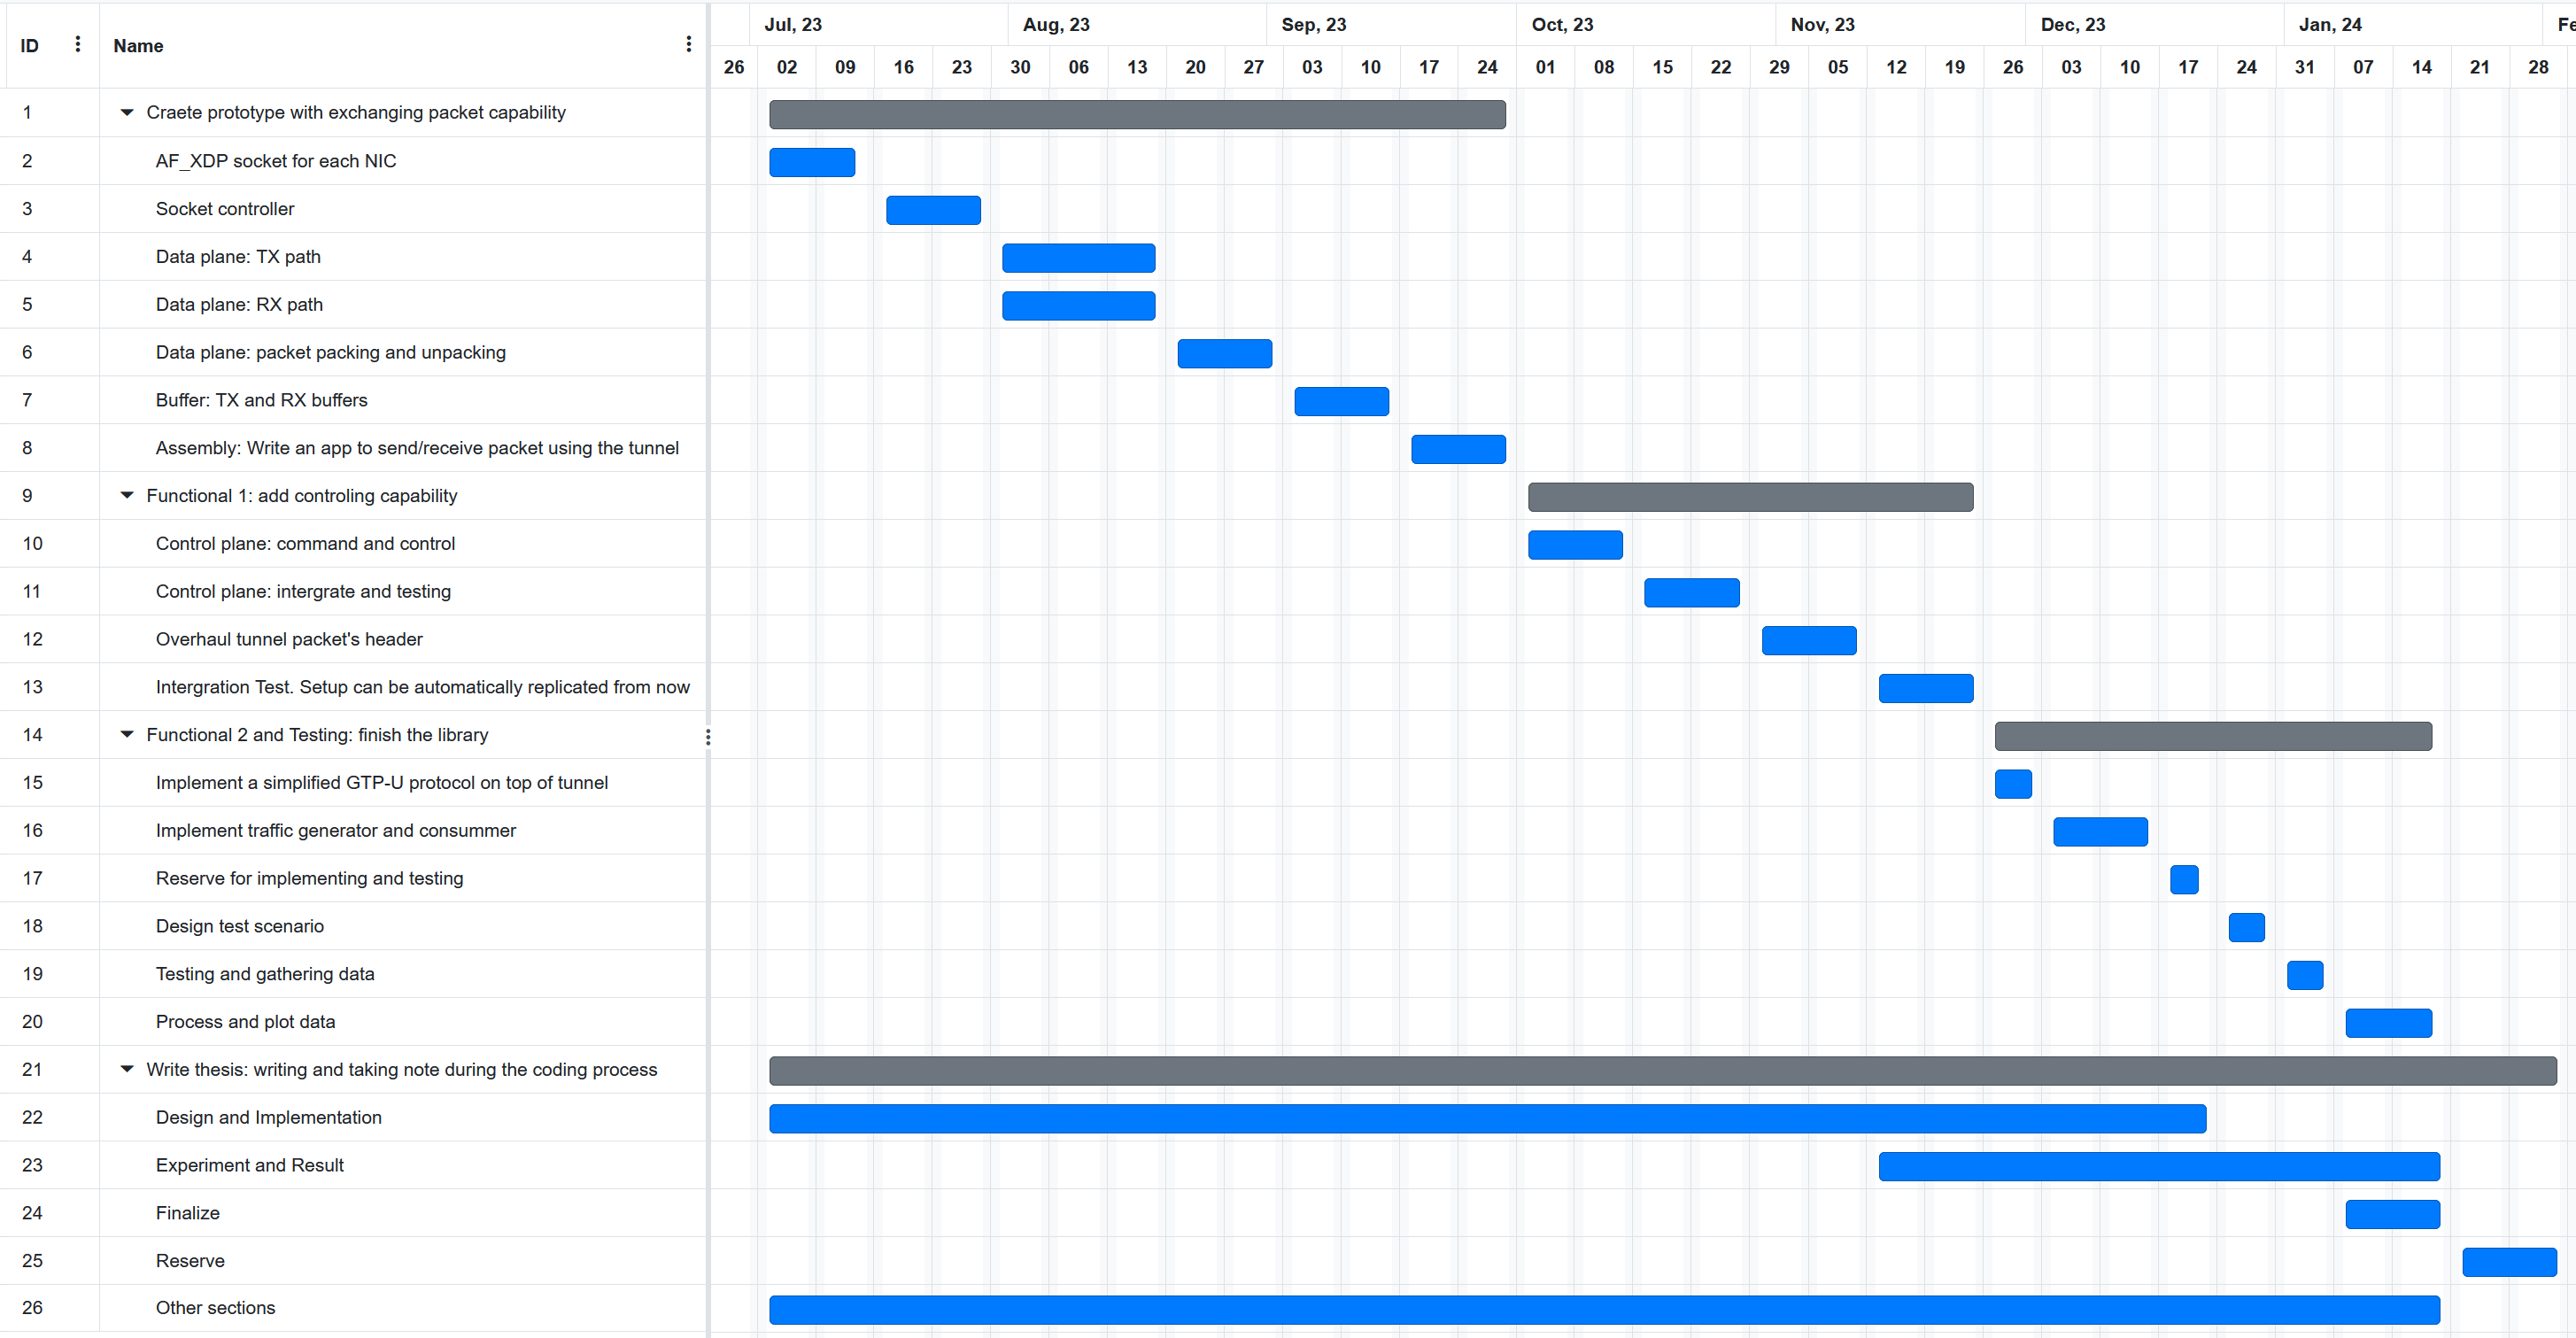
\includegraphics[width=1.0\textwidth]{resources/images/TIMELINE.PNG}
    \caption{Expected progress for the thesis project}
	\label{fig:plan:TIMELINE}
  \end{sidewaysfigure}

\clearpage
\section{Development Environment}
The development process will take place within a Linux environment. 
As for testing purposes, the program binary will be deployed and executed on 2 industrial-grade computers \textit{UP CORE} designed by \ac{AAEON}, equipped with multiple Ethernet ports \cite{upc_core} \cite{upc_extension_board}. 
The binary will establish a tunnel between two UPC machines using three specific Ethernet ports. 
It's important to note that the fourth port is unrelated to the multipath tunneling and is solely used for remote management purposes.
The UPC machines, equipped with this library, can be utilized as part of the AV's 5G test bed. 
In this setup, RAN (Radio Access Network) and Open5GS software will be installed on the UPC machines, enabling comprehensive testing and evaluation of 5G functionalities.

\begin{figure}[H]
	\centering
	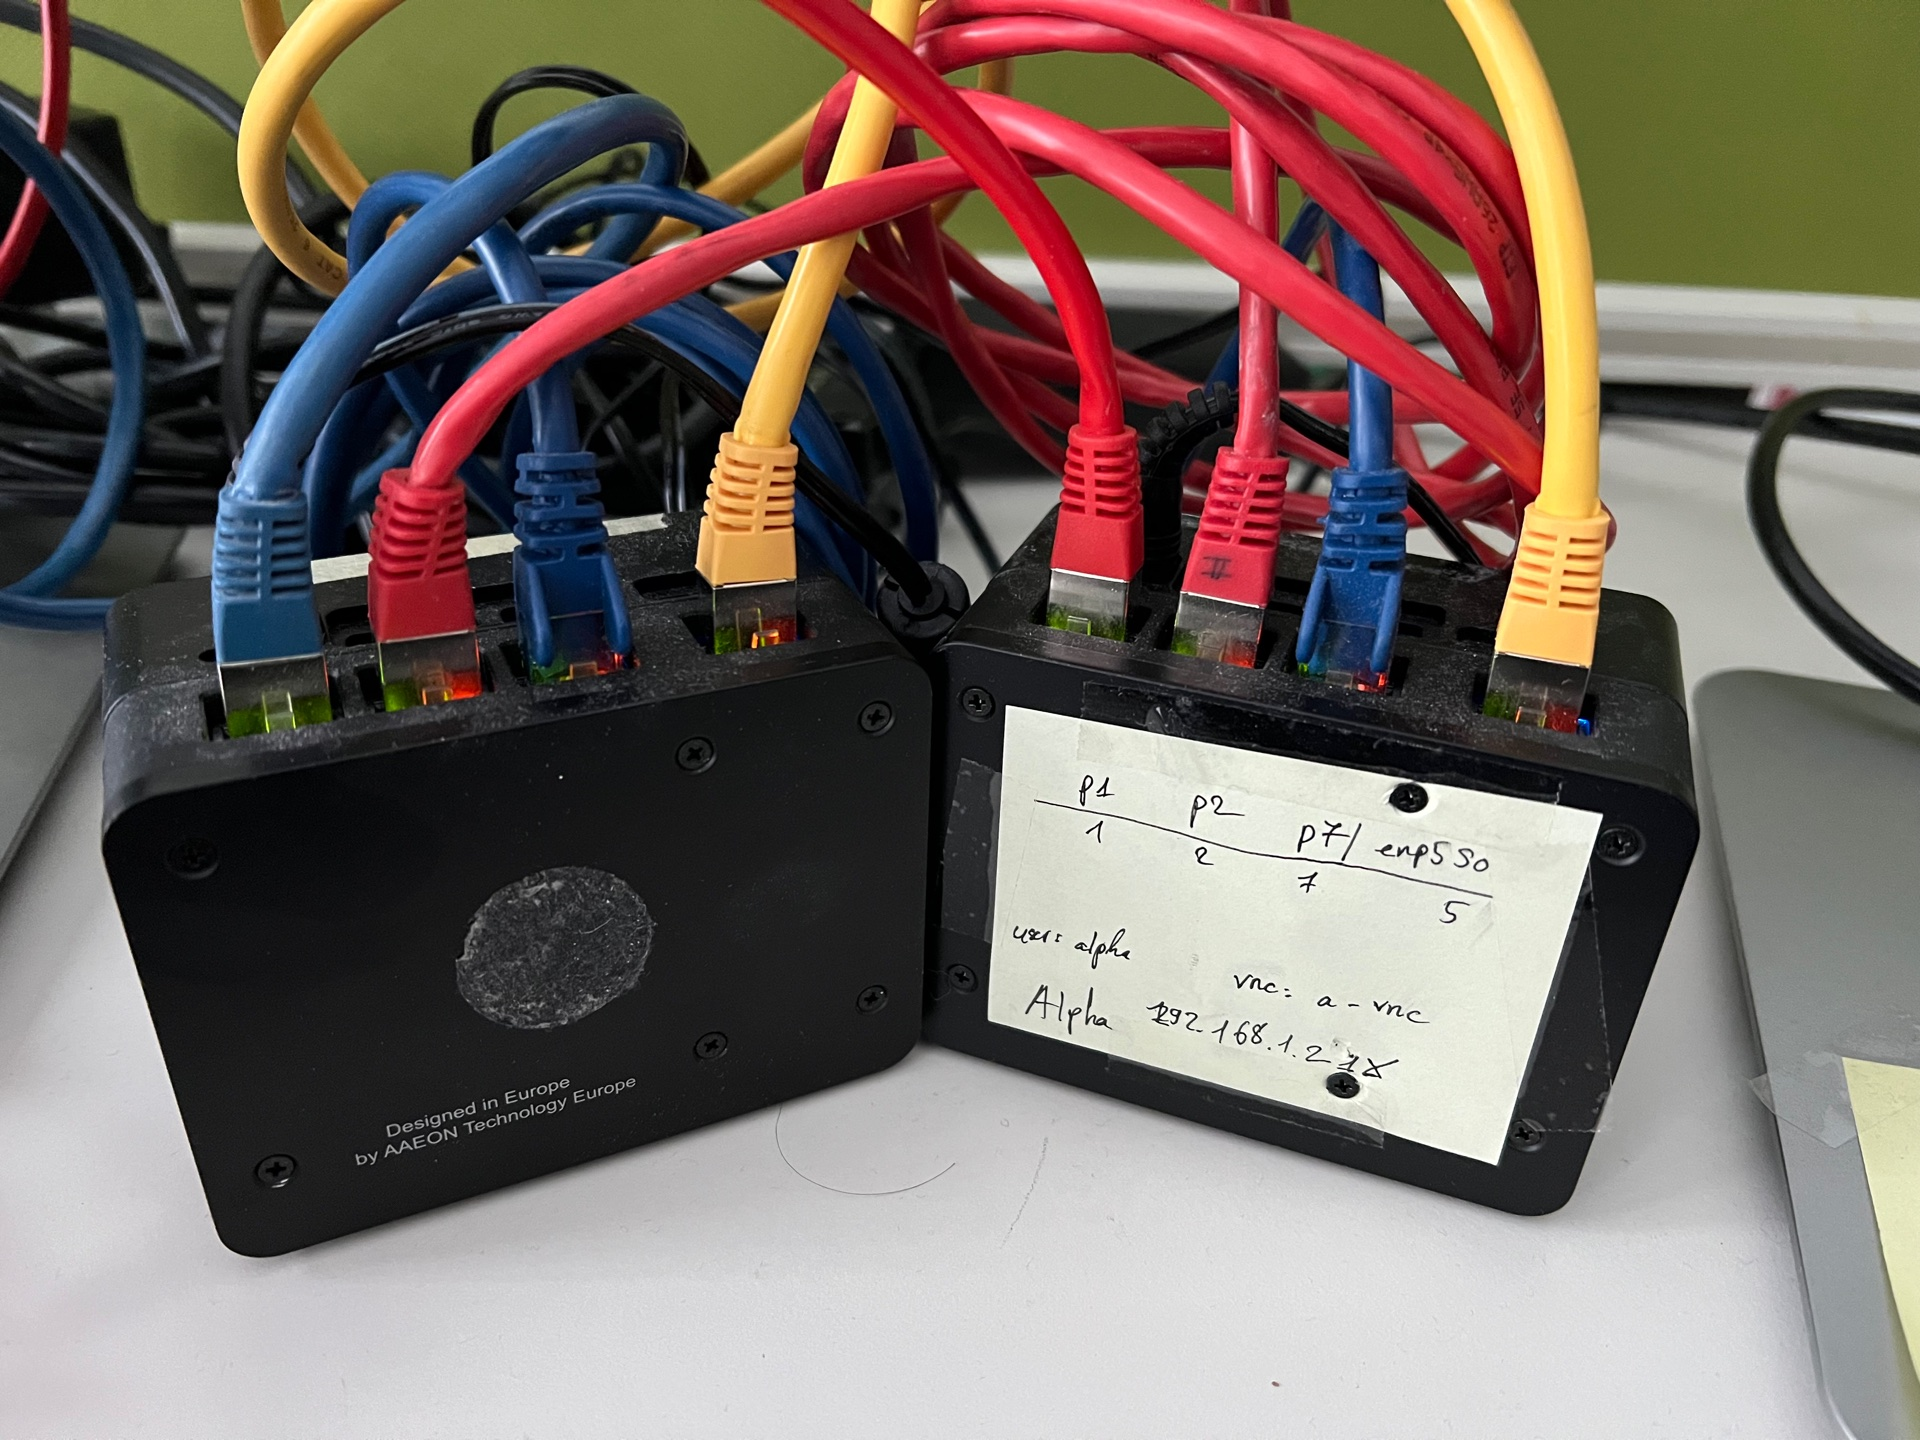
\includegraphics[width=0.8\textwidth]{upc_machines.png}
	\caption{Two UPC machines with 3 ethernet ports connected (\textit{enp3s0}, \textit{enp5s0}, \textit{enp7s0}). Port \textit{enp1s0} is connected to workstation for remote management purpose.}
	\label{fig:plan:upc_machines}
\end{figure}
